26. $\cfrac{(x-1)^2(x+3)(x-3)}{\sqrt{x+2}}\geqslant0.$ Применив метод интервалов, найдём ответ:
\begin{figure}[ht!]
\center{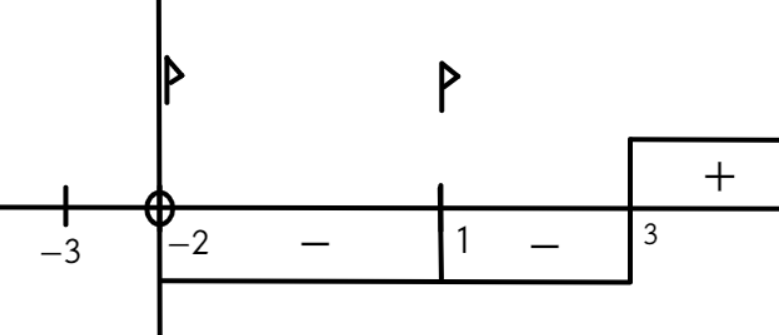
\includegraphics[scale=0.35]{int26.png}}
\end{figure}
$x\in\{1\}\cup[3;+\infty).$\newpage\noindent
